\section{Methode nach Stam}

\subsection{Motivation}

Die Methode zur approximativen Lösung der Navier-Stokes-Gleichungen, die im
Folgenden erklärt wird, wurde von \PimiddyName{Jos Stam} im Jahr 1999 entwickelt
und in dem Paper "`Stable Fluids"' vorgestellt \cite{Stam1999}. Das Verfahren
wurde speziell für die Computergrafik entwickelt, wobei auf einige
Besonderheiten eingegangen wurde:

\begin{enumerate}
\item
	Im Gegensatz zu wissenschaftlichen Simulationen ist man in der
	Computergrafik an einer Lösung interessiert, die in möglichst kurzen
	Abständen Ergebnisse produziert. Zum Beispiel möchte man die
	Strömungssimulation jedes Frame um einen Zeitschritt weiterbewegen. Um
	eine flüssige Simulation zu erhalten, ist die Laufzeit des
	Lösungsalgorithmus also auf 16 Millisekunden (für 60 Bilder pro Sekunde)
	bzw. 33 Millisekunden (für 30 Bilder pro Sekunde) beschränkt. Die
	Navier-Stokes-Gleichungen bilden als System von nichtlinearen
	Differentialgleichungen hier eine besondere Herausforderung.
\item
	Man ist außerdem nicht unbedingt an einer exakten Lösung interessiert.
	Will man z.B. Wasser oder Rauch simulieren reicht es, ein physikalisch
	annähernd korrektes Verhalten zu erzielen.
\item
	Bisherige Verfahren (wie z.B. die finiten Differenzen in
	\cite{Foster1997}) waren numerisch \emph{instabil} für große
	Zeitschritte. Dynamische Anwendungen wie Spiele oder Animationssoftware
	können allerdings keine minimiale Framerate garantieren, da sie mit
	verschiedenen Umgebungen und Hardwarekonfigurationen ausgeführt werden
	können.

	Als Ausweg muss man einen großen Zeitschritt (ein langes Frame) entweder
	ignorieren -- was die Simulation unrealistisch macht -- oder ihn in
	kleinere Zeitschritte unterteilen. Die Laufzeit des Verfahrens ist aber
	im Allgemeinen nicht von der Größe des Zeitschritts abhängig. Dies führt
	dazu, dass das nächste Frame erneut viel Rechenzeit benötigt und wieder
	entsprechend lang wird.

	Dieser Effekt ist nicht mehr aufzuhalten und die Simulation
	\PimiddyQuotes{explodiert}.
\item
	Bisherige Verfahren waren auf Hilfe des Designers angewiesen, um Teile
	der Simulation möglichst realistisch zu modellieren. Bestimmte natürlich
	vorkommende Turbulenzen mussten explizit in die Simulation eingegeben
	werden. Idealerweise sollte die Simulation allerdings von selber
	fortgeführt werden, der Designer sollte nur Rahmenbedingungen wie
	Hindernisse und globale Eigenschaften des Fluids (wie Dichte und
	Viskosität) vorgeben.
\end{enumerate}

\begin{figure}[ht]
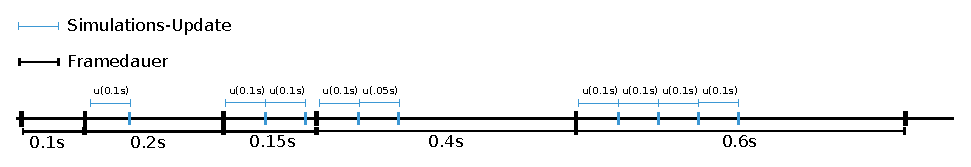
\includegraphics[width=12cm]{images/simulation_blowup}
\caption{Instabilität in Simulationen: Hier wird angenommen, die maximal zu simulierende Simulationsdauer sei $0.1s$. Längere Frames werden in mehreren Ticks berechnet, die aber konstant lange Laufzeit haben. Dies führt zu dauerhaft langen Frames, der Effekt potenziert sich.}
\end{figure}

Das Verfahren ist also auf Geschwindigkeit ausgelegt, basiert aber
nichtsdestotrotz auf den Navier-Stokes-Gleichungen und erzielt akkurate
Simulationsergebnisse. Anfängliche Schwachstellen des Verfahrens wie die zu
starke Dämpfung von Wirbeln wurden in weiteren Arbeiten ausgebessert
\cite{Foster}. Diese Verbesserungen sind teilweise auch in die Arbeit
eingeflossen.

Wegen der numerischen Stabilität und sehr guten Parallelisierbarkeit wird Stams
Verfahren bereits in einigen Spielen eingesetzt (siehe \cite{Crane2007},
\cite{Peschel2009}). Hier beschrieben wird eine leicht abgewandelte
Fassung, bei der andere Randbedingungen verwendet werden.

\subsection{Überblick über das Verfahren}

Die Fluidsimulation findet auf einem diskreten, endlichen Gitter, also einer
Teilmenge von $\PimiddyGanz^n$ statt. Gegeben sei das Geschwindigkeitsfeld zum
Zeitpunkt $t$: $\vec{u}_{i,j,k}^t$. Als Anfangsbedingung könnten zum Zeitpunkt $0$
z.B. alle Zellen auf eine vorgegebene \PimiddyQuotes{Windrichtung} gesetzt sein.
Gegeben sei außerdem ein Zeitdelta $\Delta t$ (nicht zu verwechseln mit dem
Laplaceoperator). Ziel ist es, unter Zuhilfenahme der
Navier-Stokes-Gleichungen ein neues Geschwindigkeitsfeld $\vec{u}_{i,j,k}^{t+\Delta
t}$ zu berechnen.

Außerdem berechnen wir einmalig ein \emph{Hindernisfeld} $b_{i,j,k}$. Ist $b_{i,j,k}
= 1$, dann ist diese Zelle mit einem Hindernis ausgefüllt. Ist $b_{i,j,k} = 0$,
ist die Zelle frei. Im Implementierungsteil wird erklärt, wie dieses
Hindernisfeld gefüllt wird.

Die rechte Seite Impulsgleichung \eqref{eq:navier_stokes_momentum_equation} besteht
aus mehreren Summanden:

\begin{equation}
\vec{u} \PimiddyDiv \vec{u} -
\nu \PimiddyLaplace \vec{u} +
\vec{g} -
\frac{
	1
}
{
	\rho
}
\PimiddyGrad p
\end{equation}

In Stams Verfahren wird jeder dieser Summanden als eine Operation betrachtet,
die ein Geschwindigkeitsfeld sowie eventuell weitere Eingabegrößen wie $\Delta
t$ erhält, und die ein neues Geschwindigkeitsfeld zurückgibt. Das so berechnete
neue Feld wird zur Eingabe der darauffolgenden Operation. So wird die Lösung der
Impulsgleichung in kleinere Teile zerlegt, die für sich behandelt werden können:

\begin{itemize}
\item
	Der Term
	\begin{equation}
	\vec{u} \PimiddyDiv \vec{u}
	\end{equation}
	stellt die \PimiddyBegriff{Advektion} dar. Das Vektorfeld wird entlang
	seiner eigenen Strömungsrichtung weiterbewegt. Er sei im Folgenden mit
	\PimiddyInlineCode{advection}$(\vec{u},\Delta t)$ bezeichnet.
\item
	Der Term
	\begin{equation}
	\nu \PimiddyLaplace \vec{u}
	\end{equation}
	stellt die viskose \PimiddyBegriff{Diffusion} dar. Selbst wenn keine
	Kräfte auf das Fluid wirken, bewegt es sich durch Diffusionsprozesse
	weiter, so wie Farbe auf einem Blatt Papier verläuft.

	Dieser Term kann in Stams Verfahren ignoriert werden. Diffusion entsteht
	ohnehin \PimiddyQuotes{zufällig} durch Genauigkeitsfehler während der
	Advektion (siehe unten). So kann Performance eingespart werden, denn die
	Lösung dieses Terms ist sehr aufwändig.
\item
	Der Term $\vec{g}$ umfasst schlicht das Aufsummieren aller äußeren
	Kräfte, die auf das Fluid wirken. Hierzu gehört sowohl die Schwerkraft
	als auch der von außen eingeführte Wind. Die Operation bekommt als
	Eingabe das Geschwindigkeitsfeld sowie das Zeitdelta (bei größerem
	Zeitunterschied zum letzten Simulationsschritt sollen die Kräfte
	stärker wirken). Sei sei im folgenden mit
	\PimiddyInlineCode{externalForces}$(\vec{u},\Delta t)$ bezeichnet.
\item
	Der \emph{Druck} des Fluids wird in dem Term
	\begin{equation}
	-\frac{1}{\rho} \PimiddyGrad p
	\end{equation}
	zusammengefasst. Er dient am Ende unter anderem dazu, die
	Randbedingungen und die Un"-komp"-ri"-mier"-bar"-keit zu erzwingen. Die Berechnung
	des Drucks sei mit \PimiddyInlineCode{calculatePressure}$(\vec{u})$
	bezeichnet.
\item
	Wie bei Differentialgleichungen üblich, müssen wir noch die
	\emph{Rand- und Anfangsbedingungen} behandeln. Dadurch wird
	einerseits sichergestellt, dass der das Fluid nicht in Hindernisse
	eindringt, andererseits an den Rändern der Simulation frei hinausfließen
	kann. Diese Operation wird im Folgenden als
	\PimiddyInlineCode{boundaries}$(\vec{u})$ bezeichnet und wird vor der
	Berechnung des Drucks eingefügt.
\end{itemize}

\begin{algorithm}
\caption{Der Lösungsalgorithmus in Pseudocode}
\label{alg:stam_first_algorithm}
\begin{algorithmic}
\Function{simulate}{$\vec{u}$,$\Delta t$}
	\State $\vec{u}'$ = advection($\vec{u}$,$\Delta t$)
	\State $\vec{u}''$ = externalForces($\vec{u}'$,$\Delta t$)
	\State $\vec{u}'''$ = boundaries($\vec{u}''$)
	\State $p$ = calculatePressure($\vec{u}$)
	\State \Return $\vec{u}''' - \PimiddyGrad p$
\EndFunction
\end{algorithmic}
\end{algorithm}

\begin{figure}[ht]
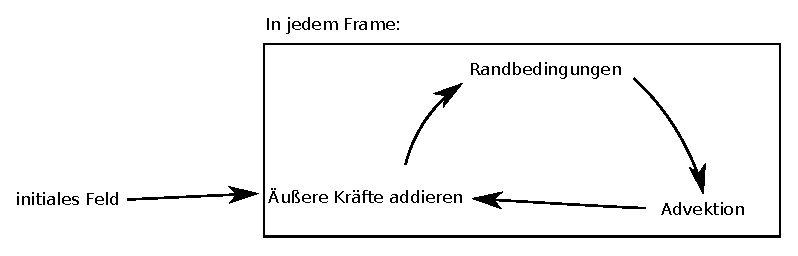
\includegraphics[width=10cm]{images/stam_loop}
\caption{Die Simulationsschleife ohne Projektion.}
\end{figure}

Für jeden Term wird im Folgenden ein Lösungsalgorithmus vorgestellt, insgesamt
erhält man den Pseudocode in \autoref{alg:stam_first_algorithm}.

\subsection{Advektion}

Wie bereits in der Erklärung der Navier-Stokes-Gleichungen angedeutet, wird bei
der Advektion das Geschwindigkeitsfeld entlang \PimiddyQuotes{sich selber}
weiterbewegt. Auf diese Weise kann sich Wind, der von einer Seite der
Simulation eingeführt wird, über den gesamten Simulationsbereich ausbreiten.
Manchmal spricht man daher auch von \emph{Selbstadvektion}. In älterer Literatur
ist auch von \emph{Konvektion} die Rede.

Im Folgenden gehen wir etwas allgemeiner davon aus, dass eine \emph{beliebige} Größe
$q_{i,j,k}^t$ entlang des Vektorfelds $\vec{u}$ bewegt werden soll. Die Methode
\PimiddyInlineCode{advection} kann also auch verwendet werden, um
Temperaturwerte oder die Dichte des Rauchs an einer Stelle entlang des
Vektorfeldes weiterzubewegen. Als Ausgabe erhalten wir ein neues Feld
$q_{i,j,k}^{t+\Delta t}$.

Um die Advektion durchzuführen gibt es mehrere Ansätze. Der gängigste arbeitet
mit der Methode der finiten Differenzen und wurde unter anderem in
\cite{Foster} benutzt. Finite Differenzen führen aber zu einem numerisch
instabilen Algorithmus. Im Gegensatz dazu soll hier zunächst ein intuitiver
Ansatz erläutert werden, der auch numerisch instabil ist und somit nicht ohne
große Einschränkungen verwendbar ist. Dieser Ansatz wird danach leicht
modifiziert, um Stabilität zu erreichen.

\begin{figure}[ht]
\centering
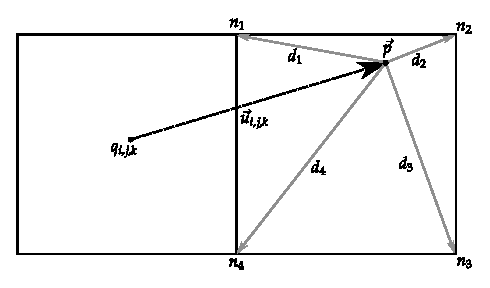
\includegraphics[width=6cm]{images/advection_bad}
\caption{Das numerisch instabile Advektionsverfahren}
\label{fig:stam_numerically_unstable_advection}
\end{figure}

Das neue Feld $q_{i,j,k}^{t+\Delta t}$ sei anfangs überall 0 (bzw. $(0,0,0)$,
falls es ein Vektorfeld ist). Man stelle sich an jedem Gitterpunkt
$(i,j,k)$ ein Partikel mit \PimiddyQuotes{Ladung} $q_{i,j,k}$ vor, was im Fluid
treibt. Durch die Bewegung des Fluids würde dieses Partikel um $\Delta t \cdot
\vec{u}_{i,j,k}$ verschoben und läge im nächsten Zeitschritt bei
$\vec{p}=(i,j,k)+\Delta t \cdot \vec{u}_{i,j,k}$. Somit läge es im Allgemeinen
nicht mehr \emph{exakt} auf einem Gitterpunkt, sondern zwischen 8 Nachbarpunkten
$n_i \in \PimiddyGanz^3, i \in \{1,\ldots,8\}$ (siehe
\autoref{fig:stam_numerically_unstable_advection}). Man bestimmt jetzt die
Distanz von $\vec{p}$ zu jedem der Nachbarpunkte:

\begin{equation}
d_i = \PimiddyNorm{2}{\vec{p} - n_i}, i \in \{1,\ldots,8\}
\end{equation}

Diese $d_i$ dienen als Gewichtung, um die \PimiddyQuotes{Ladung} $q_{i,j,k}$
anteilig auf die Nachbarknoten aufzuteilen:

\begin{equation}
q_{n_i}' \leftarrow q_{n_i}' + d_i \cdot q_{i,j,k}
\end{equation}

Dieses Verfahren ist intuitiv und einfach zu implementieren. Aber es ist
numerisch nicht stabil und führt zu Oszillationen (für eine genaue Betrachtung
sei auf die Literatur verwiesen).

Stam wählte einen anderen Ansatz, die sogenannte \emph{Methode der
Charakteristika}. Die Idee ist ähnlich zu der gerade vorgestellten, funktioniert
aber in die \PimiddyQuotes{umgekehrte Richtung}.

\begin{figure}[ht]
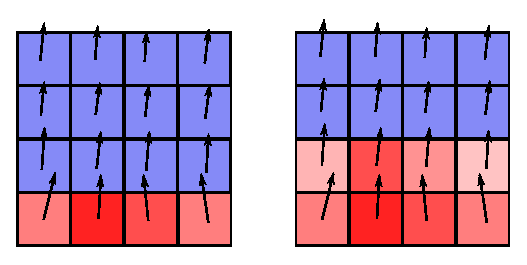
\includegraphics[width=6cm]{images/advection_bad_example}
\caption{Das numerisch instabile Advektionsverfahren für ein Temperaturfeld}
\end{figure}

Man betrachtet wieder jeden Gitterpunkt $(i,j,k)$ einzeln, stellt sich diesmal
allerdings vor, man sei auf der Zeitachse im Punkt $t+\Delta t$, also bereits im
nächsten Zeitschritt. Das (gedachte) Partikel an Position $(i,j,k)$ habe die
Geschwindigkeit $\vec{u}_{i,j,k}^t$.

Rechnet man auf der Zeitachse um $\Delta t$ zurück, erhält man die
\PimiddyQuotes{vorherige} Position des Partikels, nämlich $(i,j,k) - \Delta t
\cdot \vec{u}_{i,j,k}^t$ \PimiddyFootnote{Hier wird nur ein Schritt der
Partikelflugbahn zurückverfolgt. Es besteht die Möglichkeit, mehrere
Schritte zurückzuverfolgen, die ist aber aufwändig zu implementieren.}. Es
ergibt sich allerdings dasselbe Problem wie bei dem vorher beschriebenen Ansatz:
Diese Position liegt nicht genau auf dem Gitter, sondern dazwischen (siehe
\autoref{fig:stam_good_advection}).

Als Lösung \emph{interpolieren} wir zwischen den 8 Nachbarwerten des
verschobenen Partikels und schreiben den entstehenden Wert in die Zelle
$u_{i,j,k}^{t+\Delta t}$. Dies ist eine Operation, auf die Grafikkarten stark
optimiert sind, und bei denen traditionell Texturen hohe Performance erreichen
können.

Allerdings liegt hier auch eine Fehlerquelle des Verfahrens. Interpolation ist
eine glättende Operation, sie liefert nur eine \emph{Approximation} des Wertes,
der zwischen den Gitterzellen angenommen würde. Ähnlich wie bei der
Herleitung der diskreten Ableitung in \autoref{eq:mathematics_discretization}
muss man in der Implementierung einen Kompromiss eingehen und ein
Interpolationsverfahren wählen, was Genauigkeit und Rechenleistung verbindet.

Auch für große Zeitschritte liefert das Verfahren ein Vektorfeld als Ausgabe,
was in seinem Wertebereich beschränkt ist, denn die Interpolation liefert kein
Wert zurück, der betragsmäßig größer ist als die Ausgangswerte. Das Verfahren
ist deshalb stabil. Allerdings sollte $\Delta t$ nicht zu groß gewählt werden.
\cite{Foster} gibt hier als Richtlinie etwa $5\times$ die Gittergröße an.

\begin{figure}[ht]
\centering
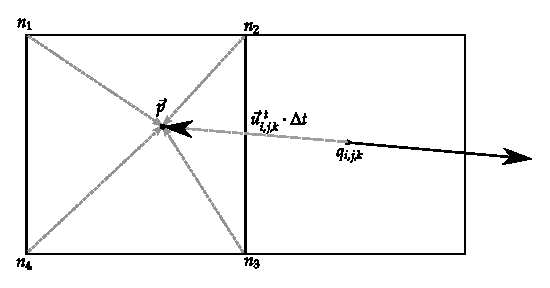
\includegraphics[width=6cm]{images/advection_good}
\caption{Stams stabiles Advektionsverfahren}
\label{fig:stam_good_advection}
\end{figure}

Natürlich kann es passieren, dass wir über den Rand des Simulationsbereiches
\PimiddyQuotes{hinauslaufen}. Es gibt mehrere Möglichkeiten, dies zu behandeln.
Beispielsweise könnte man auf die gegenüberliegenden Seite des
Simulationsbereiches umbrechen (periodische Randbedingung), was in Stams Arbeit
getan wurde. Alternativ kann man die Gerade betrachten, die durch den
Mittelpunkt der aktuellen Zelle geht, und diese Gerade mit den Rändern der
Simulation schneiden. Man wählt dann den Schnittpunkt auf dem Rand als Basis für
die Interpolation (siehe \autoref{fig:stam_clamping_borders}). Dies wurde in der
Arbeit implementiert.

\begin{figure}[ht]
\centering
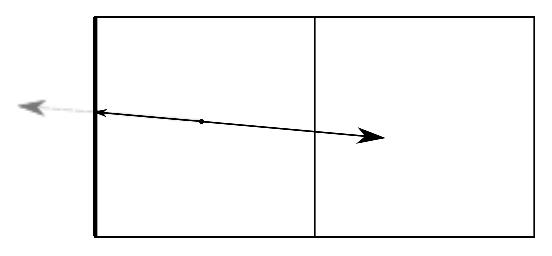
\includegraphics[width=6cm]{images/advection_clamping_borders}
\caption{Abschneiden der Geschwindigkeit an den Rändern}
\label{fig:stam_clamping_borders}
\end{figure}

Weiterhin kann der zurückberechnete Vektor $(i,j,k) - \Delta t u_{i,j,k}^t$ in
einem Hindernis landen. Man kann in diesem Fall einen Geschwindigkeitswert
von $(0,0,0)$ annehmen, was einem stationären Hindernis wie einem Gebäude
entspricht. Es ist aber auch möglich, ein weiteres Vektorfeld
$\vec{u}_{\PimiddyFormelText{boundary}}$ zu verwalten, wo für jede Gitterzelle die
\emph{Geschwindigkeit} des dort vorhandenen Hindernisses notiert ist. Dies wurde
in \cite{Crane2007} umgesetzt. Für die Simulation in dieser Arbeit wurde von
unbeweglichen Hindernissen ausgegangen.

\PimiddyTodo{Hier kurz erklären, dass das auch Semilagrangeadvektion genannt wird.}

\subsection{Äußere Kräfte}

\subsubsection{Gravitation}

Zu den äußeren Kräften gehört zu allererst die \emph{Gravitation}. Diese lässt
sich sehr einfach ausdrücken:

\begin{equation}
F_g = \Delta t (0,-9.81,0)
\end{equation}

\subsubsection{Auftrieb}

\PimiddyTodo{Auftrieb allgemein und konkret mit Buissnesq erklären}

\subsubsection{Wirbelstärkenerhaltung}

Der Advektionsschritt enthält eine lineare Interpolation, um die
Geschwindigkeitswerte in der Nachbarschaft des zurückverfolgten Partikels zu
finden. Diese simple Interpolationsmethode führt allerdings dazu, dass
Genauigkeit bei der Simulation verloren geht. Dadurch werden viele interessante
Phänomene in Fluiden, wie die starke Wirbelbildung bei Rauch, gedämpft und
treten nicht mehr so stark in Erscheinung.

Um dies auszugleichen, gibt es mehrere Ansätze. MacCormack hat ein
Advektionsverfahren entwickelt, was nicht mehr unbedingt stabil ist, aber eine
bessere Fehlerabschätzung liefert \cite{Selle2008}\cite{Crane2007}. Dadurch
entstehen mehr Wirbelphänomene, allerdings bietet diese Methode keinen Einfluss
darauf, wie stark die Wirbel auftreten sollen.

Stattdessen wurde hier eine Technik namens
\PimiddyBegriff{Wirbelstärkenerhaltung} (\PimiddyEnglisch{vorticity
confinement}) umgesetzt. Sie ist einfach zu implementieren und erlaubt,
die Stärke zu variieren.

\subsection{Projektion}

\subsubsection{Einleitung}

Die vorgestellten Al"-go"-rith"-men be"-rück"-sich"-ti"-gen die
Un"-komp"-ri"-mier"-bar"-keit des Flu"-ids nicht. Nach der Advektion und der
Addition der äußeren Kräfte kann die zweite Bedingung
\ref{eq:navier_stokes_incompressibility_condition} in den
Navier-Stokes-Gleichungen also verletzt sein, und die Simulation somit nicht
mehr physikalisch korrekt. Außerdem sind die Randbedingungen eventuell verletzt
worden. Beispielsweise wurde bei der Advektion nicht beachtet, dass das Fluid um
Hindernisse herumströmen sollte. Für beide Fälle kommt der Druck $p$ als
Korrekturterm ins Spiel.

Gegeben sei ein beliebiges Vektorfeld $\vec{u}$. Gesucht ist eine Funktion
$\PimiddyProjection$, die dieses Vektorfeld auf ein quellenfreies Vektorfeld
abbildet, also eins mit $\PimiddyDiv \vec{u} = 0$. Hierzu bedient man sich eines
Ergebnisses aus der Vektoranalysis:

\begin{PimiddySatz}[Helmholtz-Zerlegung]
Sei $\vec{u}$ ein zweimal stetig differenzierbares Vektorfeld auf einem
beschränkten Definitionsbereich, dann lässt $\vec{u}$ sich zerlegen in
ein \emph{quellenfreies} Vektorfeld $\vec{w}$ und den \emph{Gradienten}
eines Skalarfeldes $p$:

\begin{equation}
\label{eq:stam_helmholtz_equation}
\vec{u} = \vec{w} + \PimiddyGrad p
\end{equation}
\end{PimiddySatz}

\autoref{eq:stam_helmholtz_equation} soll nach $\vec{w}$ aufgelöst werden, sodass
dieses Feld für die nächste Iteration des Lösungsalgorithmus verwendet werden
kann. Das Feld $p$ ist aber ebenfalls eine Unbekannte. Um die Gleichung
aufzulösen, wendet man die Divergenz auf beide Seiten der Gleichung an und nutzt
aus, dass der Operator \emph{linear} ist. Es gilt also

\begin{equation}
\PimiddyDiv (\vec{u} + \vec{v}) = \PimiddyDiv \vec{u} + \PimiddyDiv \vec{v}
\end{equation}

Als Ergebnis erhalten wir:

\begin{equation}
\label{eq:stam_poisson_equation}
\PimiddyDiv \vec{u} = \PimiddyLaplace p
\end{equation}

Hier wurde ausgenutzt, dass $\PimiddyDiv \vec{w} = 0$ gilt. Dies ist eine
sogenannte \PimiddyBegriff{Poissongleichung}. Ihre Lösung ist ein
Standardproblem in der Physik, und im Folgenden wird ein Verfahren vorgestellt,
was \autoref{eq:stam_poisson_equation} nach $p$ auflösen kann. Mit $p$ kann man
dann durch Umstellen und Bildung des Gradienten $\vec{w}$ bestimmen:

\begin{equation}
\vec{w} = \vec{u} - \PimiddyGrad p
\end{equation}

Darauf aufbauend kann man jetzt den Operator $\PimiddyProjection$ definieren

\begin{equation}
\PimiddyProjection \colon \PimiddyReell^n \to \PimiddyReell^n
\end{equation}

als die Funktion, die ein Vektorfeld auf den quellenfreien Anteil der
Helmholtz-Zerlegung abbildet (ein Vektorfeld also quellenfrei
\PimiddyQuotes{macht}). Diese Funktion wird in der Literatur auch oft
\PimiddyBegriff{Projektion} genannt. Führt man $\PimiddyProjection$ am Ende des
Algorithmus' aus, erhält man ein unkomprimierbares Vektorfeld.

\begin{figure}[ht]
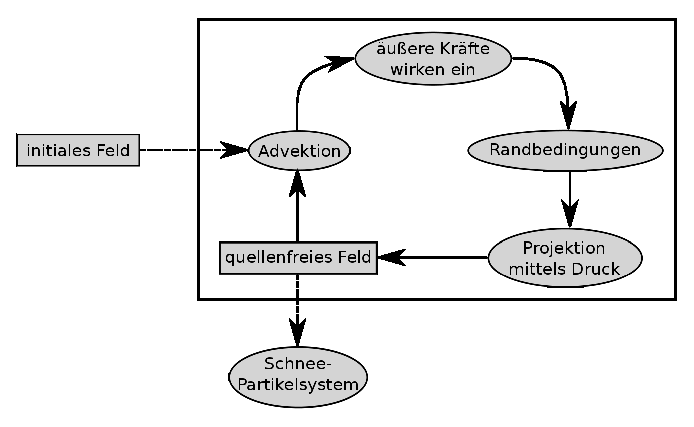
\includegraphics[width=10cm]{images/stam_loop_with_projection}
\caption{Die Simulationsschleife mit Projektion.}
\end{figure}

\subsubsection{Lösung des Poissonproblems}

Um das Vektorfeld quellenfrei zu machen, muss folgende
\PimiddyBegriff{Poissongleichung} nach $p$ gelöst werden:

\begin{equation}
\PimiddyLaplace{p} = x
\end{equation}

wobei $x$ ein Skalarfeld ist. Es existieren zahlreiche Lösungsverfahren für solch
eine Gleichung. Bei der Auswahl des Verfahrens muss beachtet werden, welches
Verfahren sich gut auf der Grafikkarte umsetzen lässt und möglichst schnell eine
ausreichend gute Lösung liefert.

Es haben sich mehrere sogenannte \PimiddyBegriff{Iterationsverfahren} als
günstig herausgestellt. Verfahren dieser Art beginnen mit einer initialen Lösung
(beispielsweise schlicht $p=0$) und nähern sich dann in jedem Iterationsschritt
weiter der eigentlichen Lösung an.

Betrachtet man große Felder, bieten sich \PimiddyBegriff{Mehrgitterverfahren}
an. Diese wurde bereits erfolgreich auf GPUs angewendet (siehe \cite{Bolz2002},
\cite{Matthias2006}). Sie sind allerdings untrivial zu implementieren, da intern
ein zweites Iterationsverfahren benötigt wird (der sogenannte
Restriktionsoperator), sowie Methoden zum hoch- und runterskalieren von
3D-Feldern.

Simplere Iterationsverfahren sind SOR (\cite{Saltvik2006}),
Gauss-Seidel-Re"-la"-xa"-ti"-on (\cite{Stam2003}) und das
Jacobiverfahren (\cite{Crane2007}, \cite{Harris2008},
\cite{Peschel2009}). Letzteres ist besonders einfach zu
implementieren und gleichzeitig hervorragend für die GPU geeignet.

\subsubsection{Das Jacobiverfahren}

Um das Jacobi-Verfahren zu veranschaulichen, soll es zunächst im
Eindimensionalen erläutert werden. Wir betrachten also kein diskretes 3D-Gitter,
sondern eine endliche Teilmenge der ganzen Zahlen (die Gitterbreite $\Delta x$
ist also $1$). Der Laplaceoperator entspricht in diesem Fall der zweiten
Ableitung von $p$.

Für die exakte Lösung $p$ des Poissonproblems muss an jeder Stelle $i$ gelten:

\begin{equation}
\label{eq:stam_jacobi_onedimensional}
\frac{
	p_{i+1} -
	2 \cdot p_{i} +
	p_{i-1}
}
{
	(\Delta x)^2
}
=
x_i
\end{equation}

Löst man diese Gleichung nach $p_i$ auf und setzt $\Delta x = 1$ ein, erhält
man:

\begin{equation}
p_i
=
\frac{
	p_{j+1} +
	p_{j-1} -
	\cdot x_i
}
{
	2
}
\end{equation}

Der Wert $p_i$ definiert sich also durch seine direkten Nachbarn $p_{i-1},
p_{i+1}$, die Gleichung ist für sich genommen nicht aufzulösen.

Sei nun eine Anfangslösung $p^0$ gegeben, z.B. $p^0_i = 0$ für alle $i$.
Dann lässt sich eine neue, bessere Lösung bestimmen, indem man die Werte aus
$p^0$ als Näherungen für die Nachbarn in der exakten Lösung nimmt:

\begin{equation}
\label{eq:stam_jacobi_onedimensional_iterative_solution}
p_i^1
=
\frac{
	p_{j+1}^{0} + p_{j-1}^{0} - x_i
}
{
	2
}
\end{equation}

Im nächsten Iterationsschritt berechnet man dann $p_i^2$ mit Hilfe von $p_i^1$,
usw., bis man nahe genug an die exakte Lösung herangekommen ist. In der Praxis
sind mindestens 20 Iterationen nötig, da das Verfahren sehr langsam konvergiert.

Eine leichte Konvergenzverbesserung erreicht man, indem man die rechte Seite von
\autoref{eq:stam_jacobi_onedimensional_iterative_solution} nicht direkt als neue
Lösung nimmt, sondern zwischen der bisherigen Lösung und der neue Lösung mit
einem Gewichtungsfaktor $\omega$ interpoliert:

\begin{align}
\overline{p}_i^{n+1}
&=
\frac{
	p_{j+1}^{n} + p_{j-1}^{n} - x_i
}
{
	2
} \\
p_i^{n+1}
&=
(1-\omega) \cdot p_i^n + \omega \cdot \overline{p}_i^{n+1}
\end{align}

Dieses Verfahren wird \PimiddyBegriff{gewichtete Jacobi-Iteration} genannt. In
der Praxis hat sich ein Faktor von $\omega=\frac{2}{3}$ als günstig erwiesen.

In drei Dimensionen ergibt sich dasselbe Schema, nur mit 6 Nachbarn:

\begin{equation*}
p_{i,j,k}^{n+1}
=
\frac{
	p_{i+1,j,k}^n +
	p_{i-1,j,k}^n +
	p_{i,j+1,k}^n +
	p_{i,j-1,k}^n +
	p_{i,j,k+1}^n +
	p_{i,j-1,k-1}^n -
	x_{i,j,k}^n
}
{
	6
}
\end{equation*}

\subsubsection{Randbedingungen in Differentialgleichungen}

Auch bei der Berechnung des Drucks müssen Randbedingungen beachtet werden. Dies
betrifft einerseits den Rand der Simulation, denn dort hat nicht jede Zelle 6
Nachbarn (an den Ecken des Würfels nur 3). Außerdem muss der Druck in
Hinderniszellen so gewählt werden, dass das Fluid nicht in das Hindernis
eindringt.

Es gibt im Wesentlichen zwei Arten von Randbedingungen bei einer
Differentialgleichung (wie der Poissongleichung),
\PimiddyBegriff{Dirichlet-Randbedingungen} und
\PimiddyBegriff{Von Neumann-Randbedingungen}:

\begin{itemize}
\item
	Bei Dirichlet-Randbedingungen wird der \emph{Wert} des Feldes am Rand
	fest vorgeschrieben. Beispielsweise könnte man die Druckwerte, die über
	den Simulationsrand hinausgehen (z.B. $p_{-1,-1,-1}$), als $0$ annehmen.
	Dies ist gewissermaßen bei der Advektion geschehen, wo die
	Geschwindigkeit bei Hinderniszellen als $(0,0,0)$ angenommen wurde.
\item
	Bei Von Neumann-Randbedingungen schreibt man die \emph{Ableitung in
	Richtung der Normalen} an einem Punkt vor:

	\begin{equation}
	\frac{
		\partial \vec{u}
	}
	{
		\partial \vec{n}
	}(x)
	=
	f(x)
	\end{equation}

	Beispielsweise könnte man $f(x)=0$ wählen. Wie bereits in
	\autoref{sec:mathematics_incompressibility_condition_section} erläutert
	bedeutet das, dass die Geschwindigkeitspfeile nicht in ein Hindernis
	hinein- oder hinauszeigen dürfen. Das Fluid darf sich aber tangential
	frei bewegen. Diese Randbedingung wird deshalb auch spezieller als
	\PimiddyBegriff{free-slip}-Randbedingung bezeichnet.
\end{itemize}

\begin{figure}[ht]
\centering
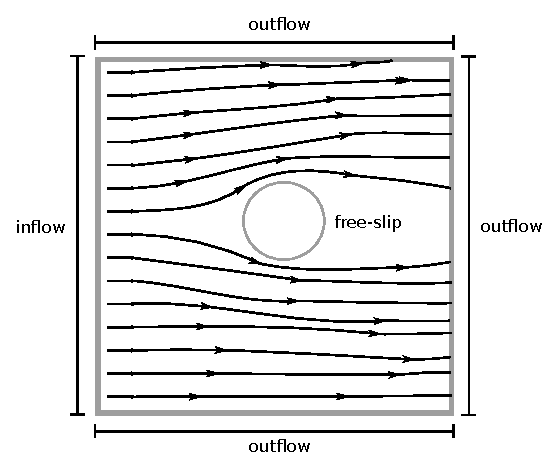
\includegraphics[width=8cm]{images/boundary_types}
\caption{Strömungslinien einer Beispielsimulation mit 3 verschiedenen Randbedingungen.}
\label{fig:stam_boundary_types}
\end{figure}

In der Simulation soll ein Teilbereich der echten Welt simuliert werden. Der
Wind wird von einigen Seiten künstlich in die Simulation gespeist. Dies nennt
man \PimiddyBegriff{inflow boundary} und ist eine Form der
Dirichlet-Randbedingung. Aus den verbleibenden Seiten soll der Wind frei aus der
Simulation \PimiddyQuotes{herausfließen}, als würde der Simulationsbereich dort
noch weitergeführt werden. Diese Art der Randbedingung nennt man
\PimiddyBegriff{outflow boundary}.

Simuliert man Rauch oder Wasser gibt es noch weitere Arten von Randbedingungen.
Die Grenze zwischen Wasseroberfläche und Luft nennt man \PimiddyBegriff{free
surface}-Randbedingung. Um diese umzusetzen müsste man $p=0$ außerhalb
des Wassers setzen. Diese Randbedingung wird hier nicht weiter beachtet.

Eine Zusammenfassung aller Randbedingungen ist in \autoref{fig:stam_boundary_types} zu sehen.

\subsubsection{Randbedingungen in der Simulation}

Es werden zuerst die Randbedingungen für die Hindernisse betrachtet. Hier sollen
\emph{free-slip}-Bedingungen erzwungen werden. Dies soll nicht explizit
hergeleitet werden, es werden nur die Veränderungen am Jacobiverfahren
beschrieben.

Im bisher beschriebenen Jacobiverfahren betrachtet man jede Zelle $p_{i,j,k}$
des Gitters und bilden die Summe über alle Nachbarzellen. Um die Randbedingungen
einfließen zu lassen, testet man, ob die Nachbarzelle von einem Hindernis
ausgefüllt ist (hier benutzen wir das Hindernisfeld $b_{i,j,k}$, was eingangs
beschrieben wurde). Gehört die Zelle zu einem Hindernis, wird nicht der
Druckwert der \emph{Nachbarzelle} zur Summe addiert, sondern der Wert der
\emph{aktuellen Zelle} (siehe \autoref{fig:stam_modified_jacobi_algorithm}
\PimiddyTodo{Wieso kann ich hier nur auf die subfigure verweisen?}). Auf
diese Weise kommt es zu keinem Druckunterschied in Richtung eines Hindernisses,
der Gradient in dieser Richtung ist also 0.  Algorithmus
\autoref{alg:stam_modified_jacobi_algorithm} zeigt den modifizierten
Algorithmus.

\begin{algorithm}
\caption{Der modifizerte Jacobi-Algorithmus}
\begin{algorithmic}
\Function{jacobi}{$p,x$}
	\State $p' = 0$
	\Comment{Ergebnisfeld ist $p'$}
	\ForAll{$(i,j,k)$}
		\State $\textrm{sum } \gets 0$
		\ForAll{Nachbarn $(i',j',k')$ von $p_{i,j,k}$}
			\If{$b_{i',j',k'} = 1$}
				\State $\textrm{sum} \gets \textrm{sum} + p_{i,j,k}$
			\Else
				\State $\textrm{sum} \gets \textrm{sum} + p_{i',j',k'}$
			\EndIf
		\EndFor
		\State $\textrm{new} = (\textrm{sum} - x_{i,j,k})/6$
		\State $p_{i,j,k}' \gets (1-\omega) \cdot p_{i,j,k} + \omega \cdot sum$
		\Comment{Gewichtete Jacobi-Iteration}
	\EndFor
	\State \Return $p'$
\EndFunction
\end{algorithmic}
\label{alg:stam_modified_jacobi_algorithm}
\end{algorithm}

\begin{figure}[ht]
\centering
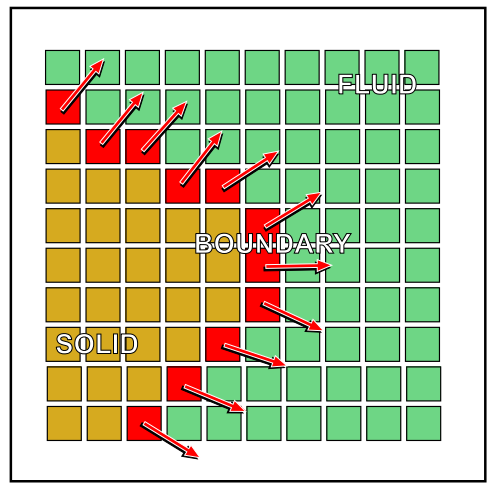
\includegraphics[width=6cm]{images/boundary_with_normals}
\caption{Hindernisse mit zugehöriger Normale}
\label{fig:stam_boundary_with_normals}
\end{figure}

Der Jacobi-Algorithmus löst die Poissongleichung allerdings nur annähernd.
Folglich werden auch die Randbedingungen nur annähernd gelöst. Dies kann im
nächsten Simulationsschritt zu Problemen führen. Daher wird in der
Implementierung die free-slip-Randbedingung nach dem Projektionsschritt
erzwungen (also nachdem der Gradient des Drucks vom Geschwindigkeitsfeld
subtrahiert wurde).

Idealerweise bräuchten wir dazu noch ein Feld $\vec{n}_{i,j,k}$, was in jedem
Punkt die Normale des Hindernisses angibt (siehe
\autoref{fig:stam_boundary_with_normals}). Dies wurde in einigen
Arbeiten umgesetzt (z.B. \cite{Bordignon}), es gibt jedoch eine Vereinfachung,
die dieses Feld nicht benötigt: Man iteriert erneut über alle
Gitterzellen und testet indem für jede Gitterzelle $(i,j,k)$, welche
Nachbarzellen von einem Hindernis ausgefüllt sind. Die zugehörige
Komponente der Geschwindigkeit $\vec{u}_{i,j,k}$ wird dann auf 0
gesetzt, siehe \autoref{alg:stam_enforce_free_slip}.

Für die outflow-Randbedingungen am Simulationsrand wird jede Randseite der
Simulation einzeln betrachtet. Die Geschwindigkeit einer Randzelle wird ersetzt
durch die Geschwindigkeit der \PimiddyQuotes{nächstinneren} Zelle.
Beispielsweise werden die Geschwindigkeitswerte $\vec{u}_{0,j,k}$ (also die an
der linken Simulationsseite) ersetzt durch die Werte $\vec{u}_{1,j,k}$. Analoges
wird für die anderen Seiten des Kubus getan, allerdings nicht dort, wo
inflow-Randbedingungen bestehen, wo also Wind in die Simulation hineinfließt.
Dadurch ergibt sich am Rand die Divergenz 0, der Druck ist hier also auch
annähernd 0 \PimiddyTodo{stimmt das überhaupt?}.

\begin{figure}[ht]
	\begin{subfigure}[b]{0.5\textwidth}
		\centering
		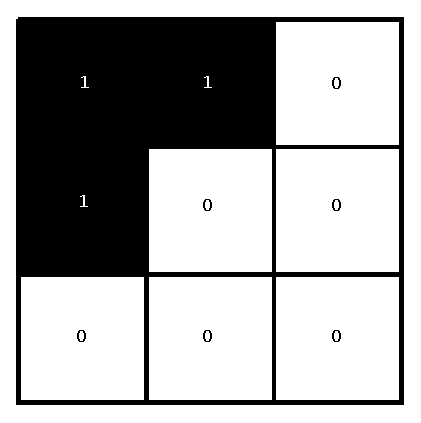
\includegraphics[width=\textwidth]{images/boundary_field_for_pressure}
		\caption{Ein beispielhaftes Hindernisfeld $b_{i,j}$}
	\end{subfigure}
	~
	\begin{subfigure}[b]{0.5\textwidth}
		\centering
		\def\svgwidth{\textwidth}
		\input{images/pressure_boundary.eps_tex}
		\caption{Die in die Druckberechnungen einfließenden Werte.}
	\label{fig:stam_modified_jacobi_algorithm}
	\end{subfigure}
\end{figure}

\begin{algorithm}
\caption{Die abschließende Randbedingungserzwingung}
\begin{algorithmic}
\Function{FreeSlipBoundary}{$\vec{v},b$}
	\ForAll{$(i,j,k)$}
		\If{$b_{i-1,j,k} = 1$ or $b_{i+1,j,k} = 1$}
			\State $\vec{u}_{i,j,k}^x = 0$
		\EndIf
		\If{$b_{i,j-1,k} = 1$ or $b_{i,j+1,k} = 1$}
			\State $\vec{u}_{i,j,k}^y = 0$
		\EndIf
		\If{$b_{i,j,k+1} = 1$ or $b_{i,j,k-1} = 1$}
			\State $\vec{u}_{i,j,k}^z = 0$
		\EndIf
	\EndFor
\EndFunction
\end{algorithmic}
\label{alg:stam_enforce_free_slip}
\end{algorithm}
